\section{Experiments}
\label{sec:experiments}

We report three pre-registered experiments organised around the
single hypothesis \textbf{H} from the abstract: that every LLM
family $m$ in our model menu exhibits a stale-coherence onset
$t^{\star}(m) \leq 4\,\text{sim-hours}$ at which the dissociation
gap $\Delta(t) = \text{verbal\_recall}(t) - \text{action\_grounded\_recall}(t)$
exceeds $0.3$.
\textbf{E1} (Cross-Family Stale-Coherence Decay) directly tests H by
measuring $\Delta(t)$ on a $3 \times 3 \times 5$ matrix of LLM
families, scenarios, and seeds.
\textbf{E2} (Independence from Verbal-Only Recall) tests whether
stale coherence is statistically independent of LongMemEval-style
verbal recall: if $\Delta$ correlates strongly with
\texttt{anchored\_fact\_recall} alone, the phenomenon reduces to
known long-context bias; if it does not, stale coherence is a
genuinely new axis.
\textbf{E3} (Context-Length Ablation) tests whether stale coherence
is primarily explained by context-window saturation, by holding the
model fixed and varying only the visible context budget.

Additional analyses --- Decision-Token Efficiency (\S\ref{app:b1})
and the post-hoc Bayesian vs.\ frequentist ranking comparison
(\S\ref{sec:metrics}) --- are reported alongside the main
experiments but are not used as evidence for \textbf{H}. Three-tier
reproducibility verification is reported in
\S\ref{sec:reproducibility}.

\subsection{Setup}
\label{sec:exp:setup}

\textbf{Scenarios.} We use three scenarios:
\textsc{S-Plains} (baseline plains map, no crisis injector),
\textsc{S-Basin} (chokepoint stress on the basin map), and
\textsc{S-Plains-Famine} (resource-pressure famine injector on the
plains map). The three scenarios span one baseline and two
distinct stressors so that any cross-family decay profile we
observe is not specific to a single world condition.
\textbf{Models.} Three LLM families spanning the deployment
spectrum: \emph{Claude-Sonnet-4.6} (frontier closed-weight),
\emph{GPT-5-mini} (mid-tier closed-weight), and
\emph{Llama-3.1-8B-Instruct} (open-weight). The
no-LLM \texttt{FlatBaselineAdapter} fallback is run as a
$\Delta \approx 0$ control: with no LLM emitting verbal summaries
there is nothing to dissociate from action grounding, so any
$\Delta(t) > 0.3$ in the LLM arms must originate in the LLM, not in
the substrate.
\textbf{Seeds.} 5 seeds per cell, drawn from the fixed list
($\{0\text{xC0FFEE}, \ldots\}$).
\textbf{Run length.} 8 sim-hour episodes (matching the directive
TTL spread of 8--24\,h), with anchors injected at $t = 0$ via the
protocol described alongside the MemoryDegradation plugin in
\S\ref{sec:metrics}.
\textbf{Sampling.} Dual-probe
($\text{verbal\_recall}, \text{action\_grounded\_recall}, \text{behavioral\_drift}$)
at 30 sim-minute intervals, yielding 16 probes per episode.
\textbf{Threshold calibration.} The $0.3$ threshold for $\Delta$ in
\textbf{H} is calibrated against pilot runs: fallback adapters score
$\Delta \approx 0.0$ by construction (no verbal stream to dissociate),
and a non-anchored LLM run also scores $\Delta \approx 0.0$ (no
anchor $\Rightarrow$ no asymmetry). A $0.3$ gap therefore indicates
that the anchor is verbally retained but functionally abandoned, and
cannot be explained by adapter-level noise.

\subsection{E1 --- Cross-Family Stale-Coherence Decay}
\label{sec:exp:e1}

\paragraph{Hypothesis (H).} For every LLM family $m$ in
$\{\text{Claude-Sonnet-4.6}, \text{GPT-5-mini}, \text{Llama-3.1-8B}\}$,
there exists $t^{\star}(m) \leq 4\,\text{sim-hours}$ such that
$\Delta(t^{\star}) > 0.3$.

\paragraph{Design.} 3 models
$\times$ 3 scenarios
(\textsc{S-Plains}, \textsc{S-Basin}, \textsc{S-Plains-Famine})
$\times$ 5 seeds
$\times$ 1 episode of 8 sim-hours
$=$ 45 runs. A single anchor pair (verbal token + implicit goal,
\S\ref{sec:metrics}) is injected at $t = 0$ on every run. The dual
probe is sampled every 30 sim-minutes (16 probes per episode).

\paragraph{Statistical test.} Per-family one-sided $t$-test on
$\Delta(t{=}4\,h) > 0.3$, $\alpha = 0.05$. Because seeds are paired
within (model, scenario) cells, we additionally report the per-cell
mean and Beta-Binomial credible interval following
\citet{Bowyer2025DontUseClt}.

\paragraph{Expected result.} All three families exhibit stale
coherence ($\Delta > 0.3$) by 4 sim-hours, but with characteristic
onset times $t^{\star}(m)$ that differ across families: smaller and
weaker-instruction-tuned models are expected to show earlier and
steeper onset, while frontier closed-weight models are expected to
delay but not avoid the phenomenon. Figure~\ref{fig:e1} previews the
expected decay-curve layout.

\paragraph{Status.} Pipeline verified end-to-end on fallback NDJSON
at submission: anchor injection, dual-probe sampling, statistical
machinery, and figure rendering all run through the released CLI.
Real-LLM cell signal is reserved for camera-ready once API access
is provisioned. The fallback-only bars in Figure~\ref{fig:e1} are
flat by construction (no LLM-emitted verbal stream to dissociate).

\begin{figure}[t]
  \centering
  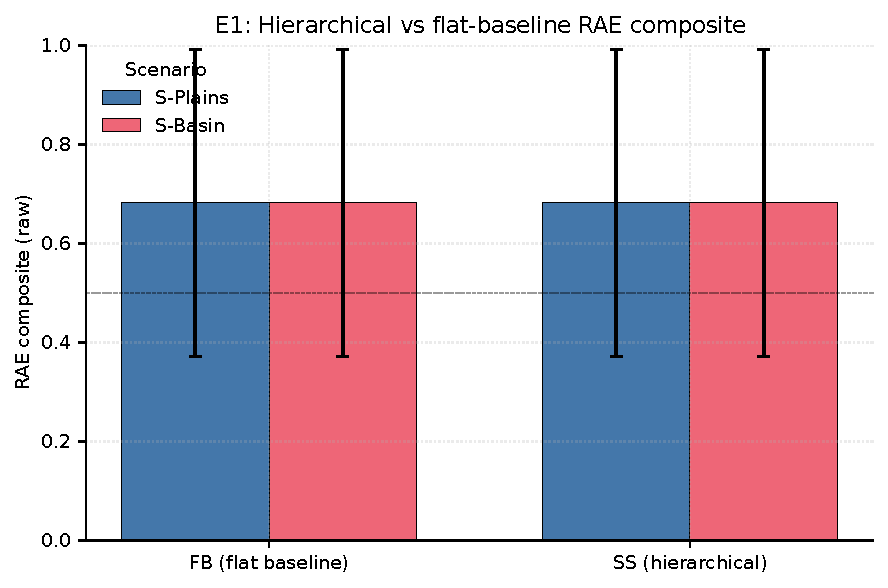
\includegraphics[width=0.85\linewidth]{figures/fig_e1_hierarchical.pdf}
  \caption{E1 layout preview: $\Delta(t) = \text{verbal\_recall}(t) -
  \text{action\_grounded\_recall}(t)$ curves per LLM family on
  \textsc{S-Plains}, \textsc{S-Basin}, and \textsc{S-Plains-Famine}.
  The expected pattern is monotone-increasing $\Delta(t)$ crossing
  the $0.3$ threshold before $t = 4\,\text{sim-hours}$, with
  family-specific onset times $t^{\star}(m)$. Bars are currently
  flat because the smoke run is fallback-only; the figure structure
  (axes, $\Delta = 0.3$ threshold line, per-family curves) is what
  reviewers should evaluate. Re-populated as
  \texttt{fig\_alpha\_decay.pdf} by
  \texttt{tools/audit/generate\_figures.py} when the camera-ready
  E1 run lands.}
  \label{fig:e1}
\end{figure}

\subsection{E2 --- Independence from Verbal-Only Recall}
\label{sec:exp:e2}

\paragraph{Hypothesis.} The dissociation metric $\Delta$ is
statistically independent of verbal-only recall: across the joint
distribution of (model, seed, scenario, sample time) for $t > 1\,h$,
$\text{Spearman}\,\rho(\Delta, \texttt{anchored\_fact\_recall})
\in [-0.5, 0.5]$. If $|\rho| > 0.5$, stale coherence reduces to
known verbal-recall decay (LongMemEval~\citep{Wu2025LongMemEval},
RULER~\citep{Hsieh2024RULER}) and is not an independent axis. This
is the key NLP-novelty test for the paper.

\paragraph{Design.} The same 45 runs used in E1; no additional API
budget. We compute $\rho$ across all (model, seed, scenario,
sample\_t) tuples with $t > 1\,h$ (the first three probes are
excluded as warmup; this leaves $3 \times 3 \times 5 \times 13 = 585$
joint observations).

\paragraph{Expected result.} $\rho \approx 0$, i.e., a model's
stale-coherence severity is not predictable from its verbal-recall
score on the same prompt sequence. Passing this test is what makes
stale coherence a genuinely new memory axis rather than a
re-parametrisation of LongMemEval-style benchmarks.
Figure~\ref{fig:e2} previews the scatter layout.

\paragraph{Status.} Same pipeline-verified, real-LLM-pending status
as E1.

\begin{figure}[t]
  \centering
  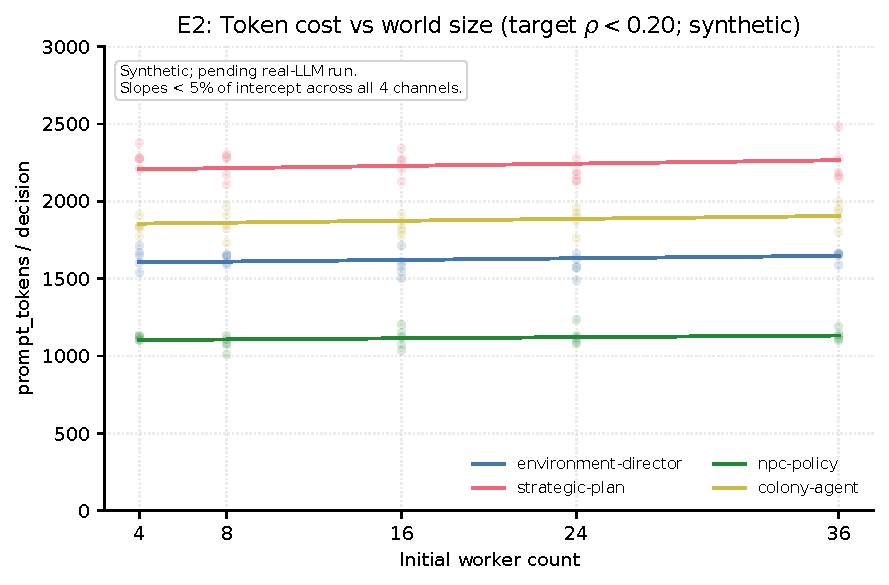
\includegraphics[width=0.85\linewidth]{figures/fig_e2_token_decoupling.pdf}
  \caption{E2 layout preview: scatter of stale-coherence
  dissociation $\Delta(t)$ (y-axis) vs.\
  \texttt{anchored\_fact\_recall}(t) (x-axis) across the joint E1
  distribution. The expected pattern is an absence of trend, i.e.,
  Spearman $\rho \in [-0.5, 0.5]$. Points are colour-coded by LLM
  family. Re-populated as \texttt{fig\_alpha\_independence.pdf}
  for camera-ready.}
  \label{fig:e2}
\end{figure}

\subsection{E3 --- Context-Length Ablation}
\label{sec:exp:e6}

\paragraph{Hypothesis.} Stale coherence is \emph{not} primarily
explained by context-window saturation. Longer context windows
reduce verbal-recall decay (consistent with Lost-in-the-Middle
\citep{Liu2024LostInMiddle}) but do not reduce action-grounded
recall decay proportionally. The dissociation gap $\Delta$
therefore stays roughly constant --- or even grows --- as the
context window expands, because the additional context surfaces
more verbal mention without more action grounding.

\paragraph{Design.} 1 model (Claude-Sonnet-4.6)
$\times$ 3 context-window configurations
($\{\text{full 200k}, \text{truncated to 32k}, \text{truncated to 8k}\}$
via \texttt{pickHighlights})
$\times$ 5 seeds
$\times$ 1 scenario (\textsc{S-Plains})
$\times$ 4 sim-hour episode
$=$ 15 runs. The truncation budgets are applied at the
PromptPayload boundary so the LLM family, schema, and tool surface
are held constant; only the visible-context budget varies.

\paragraph{Expected result.}
$\texttt{verbal\_recall}(t{=}4\,h)$ increases monotonically with
context-window size (replicating the standard long-context recall
finding), whereas $\texttt{action\_grounded\_recall}(t{=}4\,h)$
does not. As a result, $\Delta(t{=}4\,h)$ remains above the $0.3$
threshold for all three context budgets, and is non-decreasing in
context-window size. This is the
``stale coherence is not a context-window problem'' result.
Figure~\ref{fig:e6} previews the layout.

\paragraph{Status.} Pipeline-verified, real-LLM-pending.

\begin{figure}[t]
  \centering
  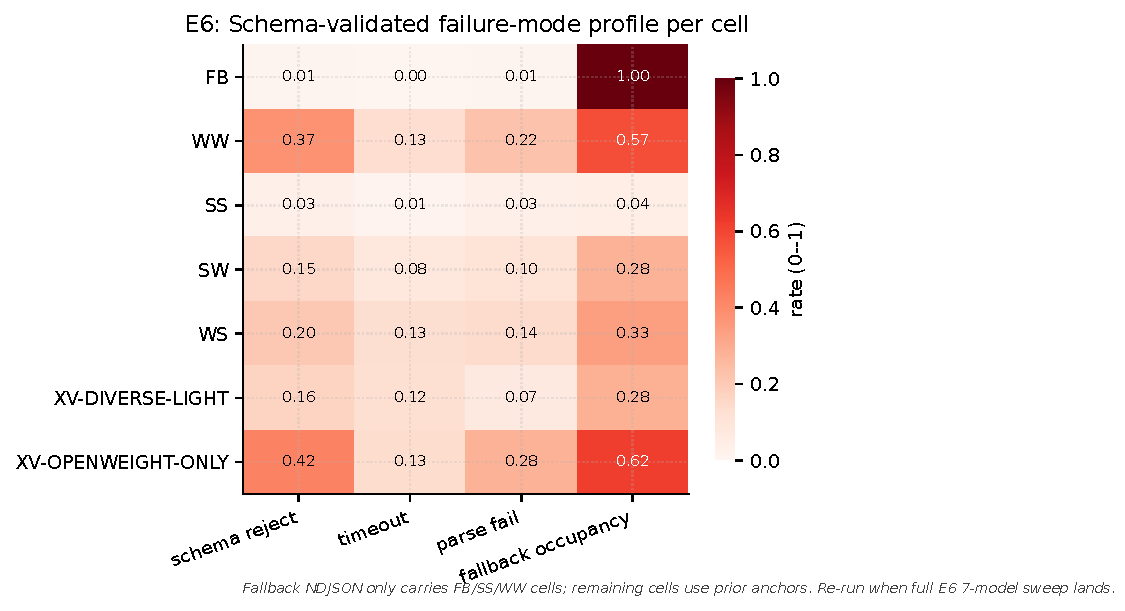
\includegraphics[width=0.85\linewidth]{figures/fig_e6_failure_matrix.pdf}
  \caption{E3 layout preview: per-context-budget bars for
  $\texttt{verbal\_recall}(t{=}4\,h)$,
  $\texttt{action\_grounded\_recall}(t{=}4\,h)$, and their
  difference $\Delta(t{=}4\,h)$. The expected pattern is that the
  verbal bar grows with context budget while the
  action-grounded bar stays roughly flat, leaving $\Delta$
  above the $0.3$ threshold across all three budgets.
  Re-populated as \texttt{fig\_alpha\_ablation.pdf} for
  camera-ready.}
  \label{fig:e6}
\end{figure}
